\chapter{Sistema di raccomandazione}
\label{cap:sistema-raccomandazione}

\intro{In questo capitolo, vengono descritte le teorie e le tecniche utilizzate per il sistema di raccomandazione, con particolare attenzione allo studio dei sistemi reali, delle tecniche di raccomandazione, di combinazione e di valutazione dei risultati. Viene inoltre dato un accenno ai temi della Serendipità e dell'Explainability, oggetto di studio del progetto sebbene non implementati allo stato dell'arte.}


\section{Requisiti per il dataset}

Perchè sia possibile implementare un sistema di raccomandazione per e-commerce, è necessario che il dataset contenga le informazioni necessarie per poter effettuare le raccomandazioni. In particolare, è necessario che il dataset contenga:
\begin{itemize}
    \item \textbf{ID Cliente}: un identificativo univoco per ogni cliente, che permette di distinguere tra i diversi clienti del servizio di e-commerce;
    \item \textbf{SKU Prodotto}: un identificativo univoco per ogni prodotto, che permette di distinguere tra i diversi prodotti del servizio di e-commerce;
    \item \textbf{Nome Cliente}: il nome del cliente, che permette di identificare quest'ultimo in modo più intuitivo; a differenza dell'ID Cliente, il nome non deve necessariamente essere univoco, cioè può essere condiviso da più clienti;
    \item \textbf{Nome Prodotto}: il nome del prodotto, che permette di identificare quest'ultimo in modo più intuitivo; a differenza dell'SKU Prodotto, il nome non deve necessariamente essere univoco, cioè può essere condiviso da più prodotti. Questo nome, nei siti di e-commerce, è generalmente molto descrittivo, e dunque non è necessario richiedere una ulteriore colonna di "descrizione".
\end{itemize}

Queste informazioni vengono dunque richieste in input come colonne del file \gls{csv} che contiene il dataset. L'\gls{llm} ha il compito di riconoscere quali colonne del file CSV ne sono rappresentanti, dopodichè i nomi corrispondenti vengono standardizzati rispettivamente in: \texttt{"Customer ID"}, \texttt{"Product SKU"}, \texttt{"Customer Name"} e \texttt{"Product Name"}. Queste colonne vengono dunque poi utilizzate per implementare le tecniche di raccomandazione, che si basano sull'analisi delle interazioni tra i clienti e i prodotti e sulla loro \gls{similarita}.

È importante notare che, per quanto il dataset possa essere grande, comunque non potrà mai contenere tutti i prodotti presenti nel magazzino del servizio di e-commerce, e dunque ci saranno sempre dei prodotti acquistabili ma ancora mai acquistati. Tuttavia, a causa dell'impossibilità di recuperare informazioni su questi ultimi, il sistema di raccomandazione si basa sulla supposizione che i prodotti già acquistati siano rappresentativi dell'intero catalogo, e dunque le raccomandazioni saranno fatte solo sui prodotti già acquistati da almeno un cliente. Questo approccio è comune nei sistemi di raccomandazione, poiché consente di fare raccomandazioni basate sulle preferenze storiche dei clienti, anche se non tutti i prodotti sono stati acquistati.
Inoltre, si fa anche la supposizione che ogni prodotto che è stato acquistato almeno una volta non abbia esaurito le scorte, e dunque sia ancora disponibile per l'acquisto. Questo è un altro presupposto comune nei sistemi di raccomandazione, quando non si hanno ulteriori dati sul magazzino.


\section{Cosine Similarity}

Prima di partire a spiegare il sistema di raccomandazione sviluppato, è importante fare una premessa, raccontando una scelta fatta in partenza che è risultata poi molto utile a seguire.

La \textbf{\gls{cosinesimilarity}}\footcite{site:cosine-similarity} è una misura di similarità particolarmente efficace per quantificare la relazione tra vettori in spazi multidimensionali, ed è stata scelta come metrica fondamentale per il sistema di raccomandazione implementato. Questa scelta è motivata da diverse considerazioni teoriche e pratiche che la rendono particolarmente adatta al contesto dei sistemi di raccomandazione.

La Cosine Similarity calcola la similarità tra due vettori $\mathbf{a}$ e $\mathbf{b}$ attraverso il coseno dell'angolo compreso tra di essi:

\begin{equation}
\text{cosine\_similarity}(\mathbf{a}, \mathbf{b}) = \frac{\mathbf{a} \cdot \mathbf{b}}{|\mathbf{a}| \cdot |\mathbf{b}|} = \frac{\sum_{i=1}^{n} a_i \cdot b_i}{\sqrt{\sum_{i=1}^{n} a_i^2} \cdot \sqrt{\sum_{i=1}^{n} b_i^2}}
\end{equation}

dove $\mathbf{a} \cdot \mathbf{b}$ rappresenta il prodotto scalare tra i due vettori, e $|\mathbf{a}|$ e $|\mathbf{b}|$ sono le rispettive norme euclidee.

Una caratteristica fondamentale della Cosine Similarity è la sua invarianza rispetto alla magnitudine dei vettori. Questa proprietà risulta particolarmente vantaggiosa nei sistemi di raccomandazione, dove è spesso necessario confrontare entità che possono avere scale di valori molto diverse. Per esempio, in un dataset di vendite, alcuni clienti potrebbero aver effettuato centinaia di acquisti mentre altri solo pochi, ma ciò che interessa è il pattern delle loro preferenze piuttosto che il volume assoluto degli acquisti.

La scelta della Cosine Similarity è inoltre supportata dalla sua ampia adozione nella letteratura sui sistemi di raccomandazione. Secondo Sarwar et al.\footcite{article:item-based-collaborative-filtering}, la Cosine Similarity rappresenta una delle metriche più utilizzate nei sistemi di Collaborative Filtering basati su item, grazie alla sua capacità di catturare efficacemente le relazioni semantiche tra prodotti indipendentemente dalla loro popolarità assoluta.

Esistono diverse alternative alla Cosine Similarity che sono state considerate durante la progettazione del sistema:

\begin{itemize}
    \item \textbf{\gls{distanzaeuclidea}}\footcite{site:euclidean_distance}: Misura la distanza geometrica diretta tra due punti nello spazio multidimensionale, ma è sensibile alla magnitudine dei vettori e può essere influenzata dalla dimensionalità;
    \item \textbf{\gls{correlazionepearson}}\footcite{site:pearson_correlation_coefficient}: Calcola la correlazione lineare tra due variabili, ma richiede che i dati seguano una distribuzione normale e può essere instabile con dati sparsi;
    \item \textbf{\gls{distanzamanhattan}}\footcite{site:manhattan_distance}: Somma delle differenze assolute tra le componenti dei vettori, semplice da calcolare ma meno efficace nel catturare relazioni complesse;
    \item \textbf{\gls{similaritajaccard}}\footcite{site:jaccard_index}: Particolarmente adatta per dati binari, misura la sovrapposizione tra insiemi, ma non considera l'intensità delle interazioni;
    \item \textbf{\gls{distanzahamming}}\footcite{site:hamming_distance}: Utilizzata principalmente per confrontare stringhe o sequenze binarie, non adatta per dati numerici continui;
    \item \textbf{\gls{divergenzakullbackleibler}}\footcite{site:kullback-Leibler_divergence}: Misura la differenza tra distribuzioni di probabilità, ma richiede che i dati siano interpretabili come distribuzioni e può essere computazionalmente costosa.
\end{itemize}

La superiorità della Cosine Similarity rispetto a queste alternative nel contesto dei sistemi di raccomandazione è documentata in diversi studi empirici. Breese et al.\footcite{article:empirical-analysis-predictive-algorithms} hanno dimostrato attraverso un'analisi comparativa che la Cosine Similarity tende a produrre risultati più stabili e accurati rispetto alla correlazione di Pearson, specialmente in presenza di dati sparsi, una caratteristica comune nei dataset di e-commerce.

Un ulteriore vantaggio della Cosine Similarity è la sua interpretabilità intuitiva: il valore risultante è sempre compreso tra -1 e 1, dove 1 indica similarità perfetta, 0 indica ortogonalità (nessuna relazione), e -1 indica opposizione completa. Questa caratteristica facilita la comprensione e la calibrazione del sistema, aspetti cruciali per la manutenibilità e l'ottimizzazione delle prestazioni.

Infine, la Cosine Similarity presenta vantaggi computazionali significativi. Il calcolo può essere ottimizzato attraverso tecniche di algebra lineare avanzate e parallelizzazione, rendendola scalabile anche per dataset di grandi dimensioni. Questa efficienza computazionale è particolarmente importante in contesti di produzione dove le raccomandazioni devono essere generate in tempo reale.

Per questi motivi, la Cosine Similarity è stata selezionata come metrica di riferimento per entrambe le tecniche di raccomandazione implementate nel sistema, garantendo coerenza metodologica e permettendo una valutazione comparativa efficace dei risultati ottenuti.



\section{Collaborative filtering}

Il primo sistema che è stato esplorato è il \textbf{Collaborative Filtering}\footcite{site:collaborative-filtering}. Questo approccio si basa sull'idea che le raccomandazioni possono essere fatte in base alle preferenze di altri utenti simili. In altre parole, se due utenti hanno gusti simili, le raccomandazioni per uno di essi possono essere utili anche per l'altro. Il Collaborative Filtering può essere implementato in due modi principali: \textbf{user-based} e \textbf{item-based}. Nel primo caso, si analizzano le preferenze degli utenti per raccomandare prodotti che altri utenti simili hanno apprezzato. Nel secondo caso, si analizzano le caratteristiche dei prodotti per raccomandare articoli simili a quelli già apprezzati dall'utente. Dopo aver svolto alcune sperimentazioni pratiche con entrambi i metodi, si è notato che i dataset disponibili contenevano spesso troppi clienti occasionali che non avevano interagito con un numero sufficiente di prodotti per poter fare raccomandazioni significative, e questo ha messo in crisi il sistema \textbf{user-based}. Inoltre, si è pensato che, in generale, per un file delle vendite di un e-commerce, sia comune la presenza di utenti occasionali. Per questo motivo, si è deciso di implementare il sistema \textbf{item-based}, che si basa sulla similarità tra i prodotti piuttosto che sulle preferenze degli utenti. Infatti, siccome i comuni dataset di vendita sono ben forniti di informazioni sui propri prodotti, questo approccio consente di fare raccomandazioni più robuste e significative.

Nel contesto del Collaborative Filtering item-based, il processo di generazione delle raccomandazioni può essere formalizzato attraverso una serie di passaggi matematici ben definiti.

\subsection{Costruzione della matrice utente-prodotto}
\label{sec:collaborative-filtering-matrice-utenti-prodotti}

Il primo passo consiste nella costruzione di una matrice di interazioni $\mathbf{F} \in \mathbb{R}^{m \times n}$, dove $m$ rappresenta il numero di utenti e $n$ il numero di prodotti. Ogni elemento $f_{ij}$ della matrice rappresenta la frequenza di interazioni (acquisti, visualizzazioni, etc.) dell'utente $i$ con il prodotto $j$:

\begin{equation}
\mathbf{F} = \begin{bmatrix}
f_{11} & f_{12} & \cdots & f_{1n} \\
f_{21} & f_{22} & \cdots & f_{2n} \\
\vdots & \vdots & \ddots & \vdots \\
f_{m1} & f_{m2} & \cdots & f_{mn}
\end{bmatrix}
\end{equation}

Nel contesto pratico del nostro sistema, gli elementi $f_{ij}$ della matrice rappresentano il numero di volte (frequenza), che l'utente $u_i$ ha acquistato il prodotto $p_j$, formalizzato come:

\begin{equation}
f_{ij} = \sum_{k \in K} \delta(u_k = i \land p_k = j)
\end{equation}

dove $K$ rappresenta l'insieme di tutti gli ordini nel dataset, $u_k$ e $p_k$ sono rispettivamente l'utente e il prodotto associati all'ordine $k$-esimo, e $\delta$ è la funzione indicatrice che vale 1 se la condizione è verificata (cioè se l'ordine $k$ è stato effettuato dall'utente $i$ per il prodotto $j$), 0 altrimenti. In questo modo, ogni elemento della matrice conta il numero totale di interazioni (acquisti) tra uno specifico utente e uno specifico prodotto.

\subsection{Calcolo della matrice di similarità prodotto-prodotto}

La matrice di similarità $\mathbf{S} \in \mathbb{R}^{n \times n}$ viene calcolata utilizzando la similarità coseno tra i vettori prodotto. Ogni prodotto $j$ è rappresentato dal vettore colonna $\mathbf{f}_j = [f_{1j}, f_{2j}, \ldots, f_{mj}]^T$. La similarità coseno tra due prodotti $j$ e $k$ è definita come:

\begin{equation}
s_{jk} = \frac{\mathbf{f}_j \cdot \mathbf{f}_k}{|\mathbf{f}_j| \cdot |\mathbf{f}_k|} = \frac{\sum_{i=1}^{m} f_{ij} \cdot f_{ik}}{\sqrt{\sum_{i=1}^{m} f_{ij}^2} \cdot \sqrt{\sum_{i=1}^{m} f_{ik}^2}}
\end{equation}

La matrice di similarità risultante è simmetrica: $\mathbf{S} = \mathbf{S}^T$.

Poi, per evitare distorsioni nelle predizioni, la matrice di similarità viene normalizzata dividendo ogni elemento per la somma delle similarità assolute della rispettiva riga:

\begin{equation}
s_{jk}^{norm} = \frac{s_{jk}}{\sum_{l=1}^{n} |s_{jl}|}
\end{equation}

ottenendo così la matrice normalizzata $\mathbf{S}^{norm}$.

\subsection{Predizione della matrice utente-prodotto}

Infine, la matrice delle predizioni $\mathbf{P} \in \mathbb{R}^{m \times n}$ viene calcolata come:

\begin{equation}
\mathbf{P} = \mathbf{F} \cdot (\mathbf{S}^{norm})^T
\end{equation}

Ogni elemento $p_{ij}$ rappresenta il punteggio predetto per l'utente $i$ rispetto al prodotto $j$, calcolato come combinazione pesata delle interazioni passate dell'utente con prodotti simili:

\begin{equation}
p_{ij} = \sum_{k=1}^{n} f_{ik} \cdot s_{kj}^{norm}
\end{equation}

Questo approccio consente di generare raccomandazioni personalizzate basate sulla similarità tra prodotti e sulle preferenze storiche degli utenti.


\section{Similarità}

Il secondo sistema che è stato esplorato è la \textbf{Similarità}. Questo approccio si basa sull'idea che le raccomandazioni possono essere fatte in base, appunto, alla similarità tra i prodotti. In altre parole, se due prodotti sono simili, le raccomandazioni per uno di essi possono essere utili anche per l'altro. La Similarità può essere implementata in diversi modi, ma il più comune è il \textbf{Cosine Similarity}\footcite{site:cosine-similarity}, che misura la similarità tra due vettori in uno spazio multidimensionale. Nel contesto del sistema di raccomandazione, i vettori rappresentano le caratteristiche dei prodotti e la similarità viene calcolata in base alla loro distanza angolare.

La tecnica di Similarità si basa sul confronto dei nomi dei prodotti, poichè nei siti di e-commerce questi ultimi sono generalmente molto descrittivi, cioè contengono molte informazioni semantiche, e non è dunque necessario richiedere una ulteriore colonna di "descrizione".

La costruzione della matrice di similarità si articola in diversi passaggi matematici fondamentali.

\subsection{Mappatura prodotto-nome}

Il primo passo consiste nella costruzione di una funzione di mappatura $\phi: \mathcal{P} \rightarrow \mathcal{N}$ che associa ad ogni prodotto $p \in \mathcal{P}$ il suo nome rappresentativo $n \in \mathcal{N}$:

\begin{equation}
\phi(p_j) = n_j \quad \forall p_j \in \mathcal{P}
\end{equation}

dove $\mathcal{P}$ rappresenta l'insieme degli identificativi dei prodotti e $\mathcal{N}$ l'insieme dei nomi dei prodotti.

\subsection{Costruzione della matrice di frequenza utente-prodotto}

Analogamente al Collaborative Filtering, si costruisce la matrice di frequenza $\mathbf{F} \in \mathbb{N}^{m \times n}$, come descritto nella sezione \S\ref{sec:collaborative-filtering-matrice-utenti-prodotti}, in cui ogni elemento $f_{ij}$ rappresenta il numero di interazioni dell'utente $i$ con il prodotto $j$.

\subsection{Calcolo della matrice di similarità semantica}

I nomi dei prodotti vengono trasformati in rappresentazioni vettoriali dense attraverso un \gls{modelloembedding} semantico $\psi: \mathcal{N} \rightarrow \mathbb{R}^d$. Ogni nome $n_j = \phi(p_j)$ viene mappato in un vettore numerico di dimensione $d$, ottenendo così il vettore di embedding $\mathbf{e}_j = \psi(n_j) \in \mathbb{R}^d$ per ogni prodotto $p_j$.

Poi, la matrice di similarità $\mathbf{S}_{sem} \in \mathbb{R}^{n \times n}$ viene calcolata utilizzando la similarità coseno tra gli embeddings dei nomi dei prodotti:

\begin{equation}
s_{jk}^{sem} = \frac{\mathbf{e}_j \cdot \mathbf{e}_k}{|\mathbf{e}_j| \cdot |\mathbf{e}_k|} = \frac{\sum_{l=1}^{d} e_{jl} \cdot e_{kl}}{\sqrt{\sum_{l=1}^{d} e_{jl}^2} \cdot \sqrt{\sum_{l=1}^{d} e_{kl}^2}}
\end{equation}

Questo approccio si distingue dal Collaborative Filtering tradizionale in quanto la similarità viene calcolata direttamente sui contenuti semantici dei nomi dei prodotti piuttosto che sui pattern di interazione degli utenti.

\subsection{Predizione della matrice utente-prodotto}

La matrice delle predizioni $\mathbf{P}_{sem} \in \mathbb{R}^{m \times n}$ viene calcolata come prodotto matriciale tra la matrice di frequenza e la matrice di similarità semantica:

\begin{equation}
\mathbf{P}_{sem} = \mathbf{F} \cdot \mathbf{S}_{sem}
\end{equation}

Ogni elemento $p_{ij}^{sem}$ rappresenta il punteggio predetto per l'utente $i$ rispetto al prodotto $j$, calcolato come:

\begin{equation}
p_{ij}^{sem} = \sum_{k=1}^{n} f_{ik} \cdot s_{kj}^{sem}
\end{equation}

Questo metodo sfrutta la ricchezza semantica dei nomi dei prodotti per identificare relazioni di similarità che potrebbero non emergere dall'analisi delle sole interazioni comportamentali, permettendo raccomandazioni più robuste anche in presenza di dati sparsi.


\section{Rank fusion}

Siccome entrambi i sistemi di raccomandazione esplorati (Collaborative Filtering e Similarità) si sono rivelati in grado di generare risultati significativi, si è deciso, invece di doverne scegliere uno, di implementarli entrambi e di combinarli in un unico sistema di raccomandazione. Per fare ciò, si è scelto di utilizzare una tecnica del \gls{rankfusion}, che consente di combinare i risultati di più sistemi di raccomandazione in un unico ranking.
Dunque, mentre le matrici sono state generate nella task di analisi delle vendite, il sistema di rank fusion è stato implementato nella task di raccomandazione, per combinare le predizioni svolte dalle due matrici.

In particolare, per la rank fusion sono state valutate diverse opzioni:
\begin{itemize}
    \item \textbf{\gls{rrf}}\footcite{article:reciprocal_rank_fusion}: Combina i ranking assegnando punteggi basati sul reciproco della posizione di ciascun elemento, favorendo gli elementi che appaiono in posizioni elevate in più sistemi;
    \item \textbf{\gls{bordacount}}\footcite{site:borda_count}: Assegna punti decrescenti basati sulla posizione nel ranking (es. n-1 punti al primo, n-2 al secondo, etc.) e somma i punti ottenuti da ciascun sistema;
    \item \textbf{\gls{scorebasednorm}}\footcite{site:score_normalization}: Normalizza i punteggi dei diversi sistemi per renderli confrontabili, quindi li aggrega tramite media pesata o altre funzioni di combinazione;
    \item \textbf{\gls{score_combination}}\footcite{article:score_combination}: Metodi che combinano i punteggi dei sistemi tramite somma (SUM), massimo (MAX), minimo (MIN) o media dei punteggi non-zero (ANZ);
    \item \textbf{\gls{weightedrank}}\footcite{article:weighted_rank_aggregation}: Combina i ranking assegnando pesi diversi ai sistemi in base alla loro affidabilità o performance, privilegiando i sistemi più performanti;
    \item \textbf{\gls{medianrank}\footcite{site:median} / \gls{geometricmeanrank}\footcite{site:geometric_mean}}: Utilizza la mediana o la media geometrica delle posizioni di ciascun elemento nei diversi ranking per determinare la posizione finale;
    \item \textbf{\gls{learningtorank}}\footcite{site:learning_to_rank}: Applica algoritmi di machine learning per apprendere la migliore combinazione dei ranking basandosi su dati di training e feedback degli utenti;
    \item \textbf{\gls{concordetfusion}}\footcite{site:condorcet_method}: Basato sul principio di Condorcet, confronta ogni coppia di elementi determinando quale è preferito dalla maggioranza dei sistemi di raccomandazione;
    \item \textbf{\gls{rbpfusion}}\footcite{article:rank_biased_precision}: Combina i ranking dando maggiore peso alle posizioni iniziali, seguendo il principio che gli utenti guardano principalmente i primi risultati.
\end{itemize}

Dietro consiglio del tutor aziendale, per la rank fusion si è scelto di utilizzare il metodo Reciprocal Rank Fusion (RRF)\footcite{site:rrf-explained}, che si basa sull'idea di assegnare un punteggio a ciascun prodotto in base al reciproco della sua posizione nei ranking dei diversi sistemi di raccomandazione. In questo modo, i prodotti che appaiono in posizioni più alte nei ranking dei diversi sistemi ottengono un punteggio più alto, mentre quelli che appaiono in posizioni più basse ottengono un punteggio più basso.

Il metodo RRF combina i ranking provenienti da diversi sistemi di raccomandazione attraverso una formula matematica ben definita. Dati $k$ sistemi di raccomandazione, ciascuno dei quali produce un ranking $rank_i$ per un determinato utente, il punteggio RRF per un prodotto $p$ è calcolato come:

\begin{equation}
\text{RRF}(p) = \sum_{i=1}^{k} \frac{1}{\text{rank}_i(p) + \rho}
\end{equation}

dove:
\begin{itemize}
    \item $\text{rank}_i(p)$ rappresenta la posizione del prodotto $p$ nel ranking del sistema $i$-esimo (con $\text{rank}_i(p) = 1$ per il primo elemento);
    \item $\rho$ è un parametro di regolarizzazione (tipicamente $\rho = 60$) che evita la divisione per zero e riduce l'impatto delle posizioni più alte;
    \item $k$ è il numero totale di sistemi di raccomandazione da combinare.
\end{itemize}

Nel contesto specifico del nostro sistema, dove $k = 2$ (Collaborative Filtering e Similarità) e $\rho = 0$ (la regolarizzazione è stata valutata come non necessaria), la formula diventa:

\begin{equation}
\text{RRF}(p) = \frac{1}{\text{rank}_{CF}(p)} + \frac{1}{\text{rank}_{Sim}(p)}
\end{equation}

Il ranking finale viene ottenuto ordinando tutti i prodotti in ordine decrescente rispetto al loro punteggio RRF. Questo approccio garantisce che i prodotti che ottengono buone posizioni in entrambi i sistemi ricevano punteggi più alti, mentre quelli che performano bene in un solo sistema mantengono comunque un punteggio significativo.

La robustezza del metodo RRF deriva dal fatto che non richiede la calibrazione dei punteggi tra i diversi sistemi, lavorando esclusivamente sui ranking ordinali, e dalla sua capacità di bilanciare automaticamente il contributo di ciascun sistema indipendentemente dalle loro scale di punteggio originali. Quest'ultima caratteristica è però un'arma a doppio taglio, poichè se in un singolo sistema un determinato prodotto ha un punteggio enormemente più alto rispetto a tutti gli altri, questo non viene considerato usando il metodo RRF, che si basa solo sulle posizioni dei prodotti nei ranking, ed allora tale prodotto non riceve il vantaggio che merita.

La seguente immagine \ref{fig:rank-fusion-toy-case} mostra un esempio di un caso giocattolo che sfrutta il metodo RRF per "fondere" due rankings.

\begin{figure}[h]
    \centering
    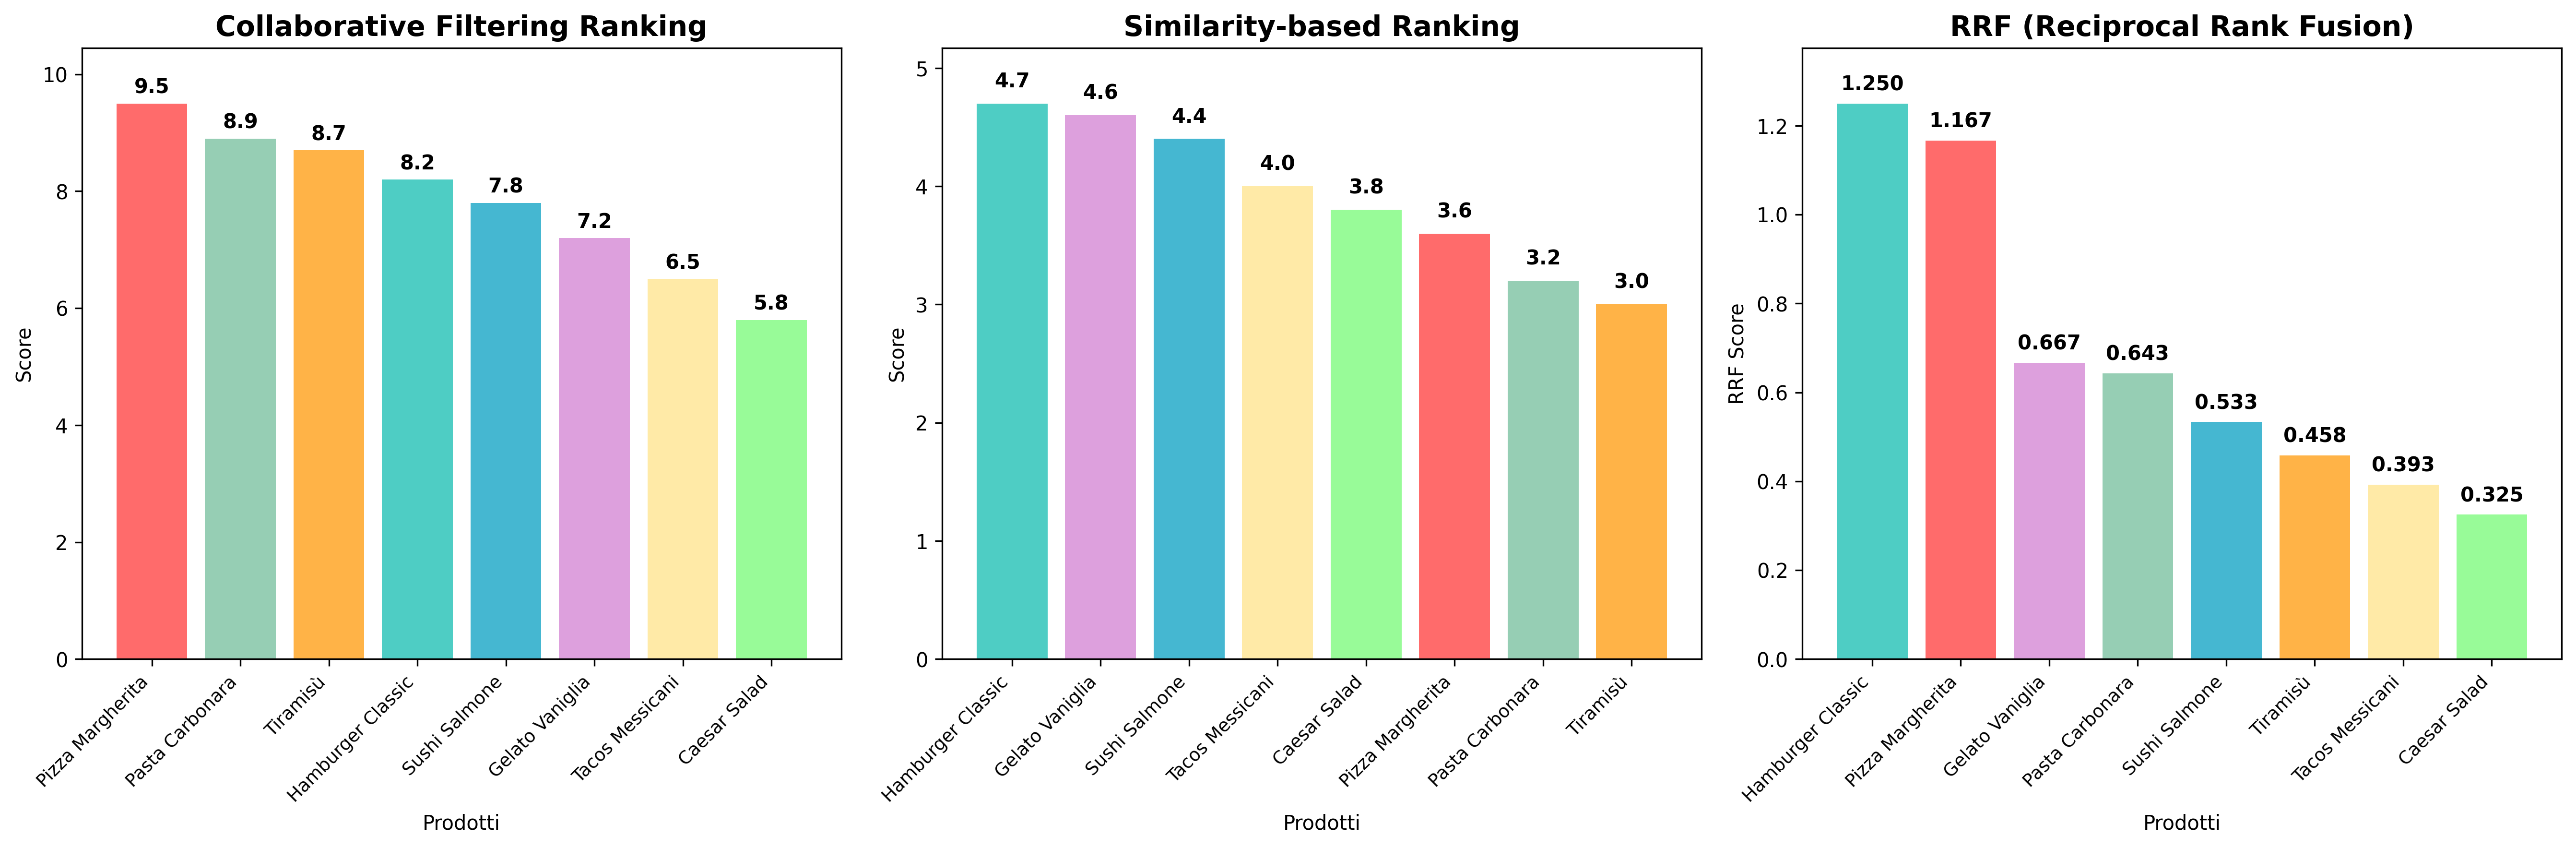
\includegraphics[width=0.8\textwidth]{rrf comparison charts/rrf_comparison_charts_toy_case.png}
    \caption{Esempio di Rank Fusion con RRF}
    \label{fig:rank-fusion-toy-case}
\end{figure}

Si può notare come tutti e 8 i prodotti siano rappresentati in tutti i rankings con lo stesso colore, per indicare che sono gli stessi prodotti, ma con posizioni diverse.
Il terzo ranking è il risultato della fusione dei primi due rankings, e mostra come i prodotti siano stati riorganizzati in base al loro punteggio RRF.

In particolare, considerando il prodotto "Hamburger Classic", il calcolo che viene fatto per il suo punteggio RRF è il seguente:

\begin{equation}
\text{RRF}(p) = \frac{1}{\text{rank}_{CF}(p)} + \frac{1}{\text{rank}_{Sim}(p)} = \frac{1}{4} + \frac{1}{1} = 1.25
\end{equation}

Oppure, considerando il prodotto "Pasta Carbonara", il calcolo che viene fatto per il suo punteggio RRF è il seguente:

\begin{equation}
\text{RRF}(p) = \frac{1}{\text{rank}_{CF}(p)} + \frac{1}{\text{rank}_{Sim}(p)} = \frac{1}{2} + \frac{1}{7} \approx 0.643
\end{equation}

E così via per gli altri prodotti. Si può notare come, nonostante i due rankings di partenza abbiano scale di punteggio diverse ("da 1 a 10" e "da 1 a 5"), il metodo RRF riesce a combinarli in modo efficace, poichè restituisce un ranking finale che tiene conto solo delle loro posizioni relative.

Al termine del processo di Rank Fusion, il sistema di raccomandazione restituisce un ranking finale dei prodotti, ordinato in base ai punteggi RRF calcolati. Questo ranking rappresenta dunque le raccomandazioni finali del sistema, che possono essere presentate agli utenti come suggerimenti personalizzati.

Un esempio di caso reale tratto dal dataset \texttt{Orders\_export.csv} è mostrato nella seguente immagine \ref{fig:rank-fusion-real-case}, che mostra i primi 10 prodotti raccomandati per il cliente \texttt{Ds-trading srl Ds-trading GmbH}.

\begin{figure}[h]
    \centering
    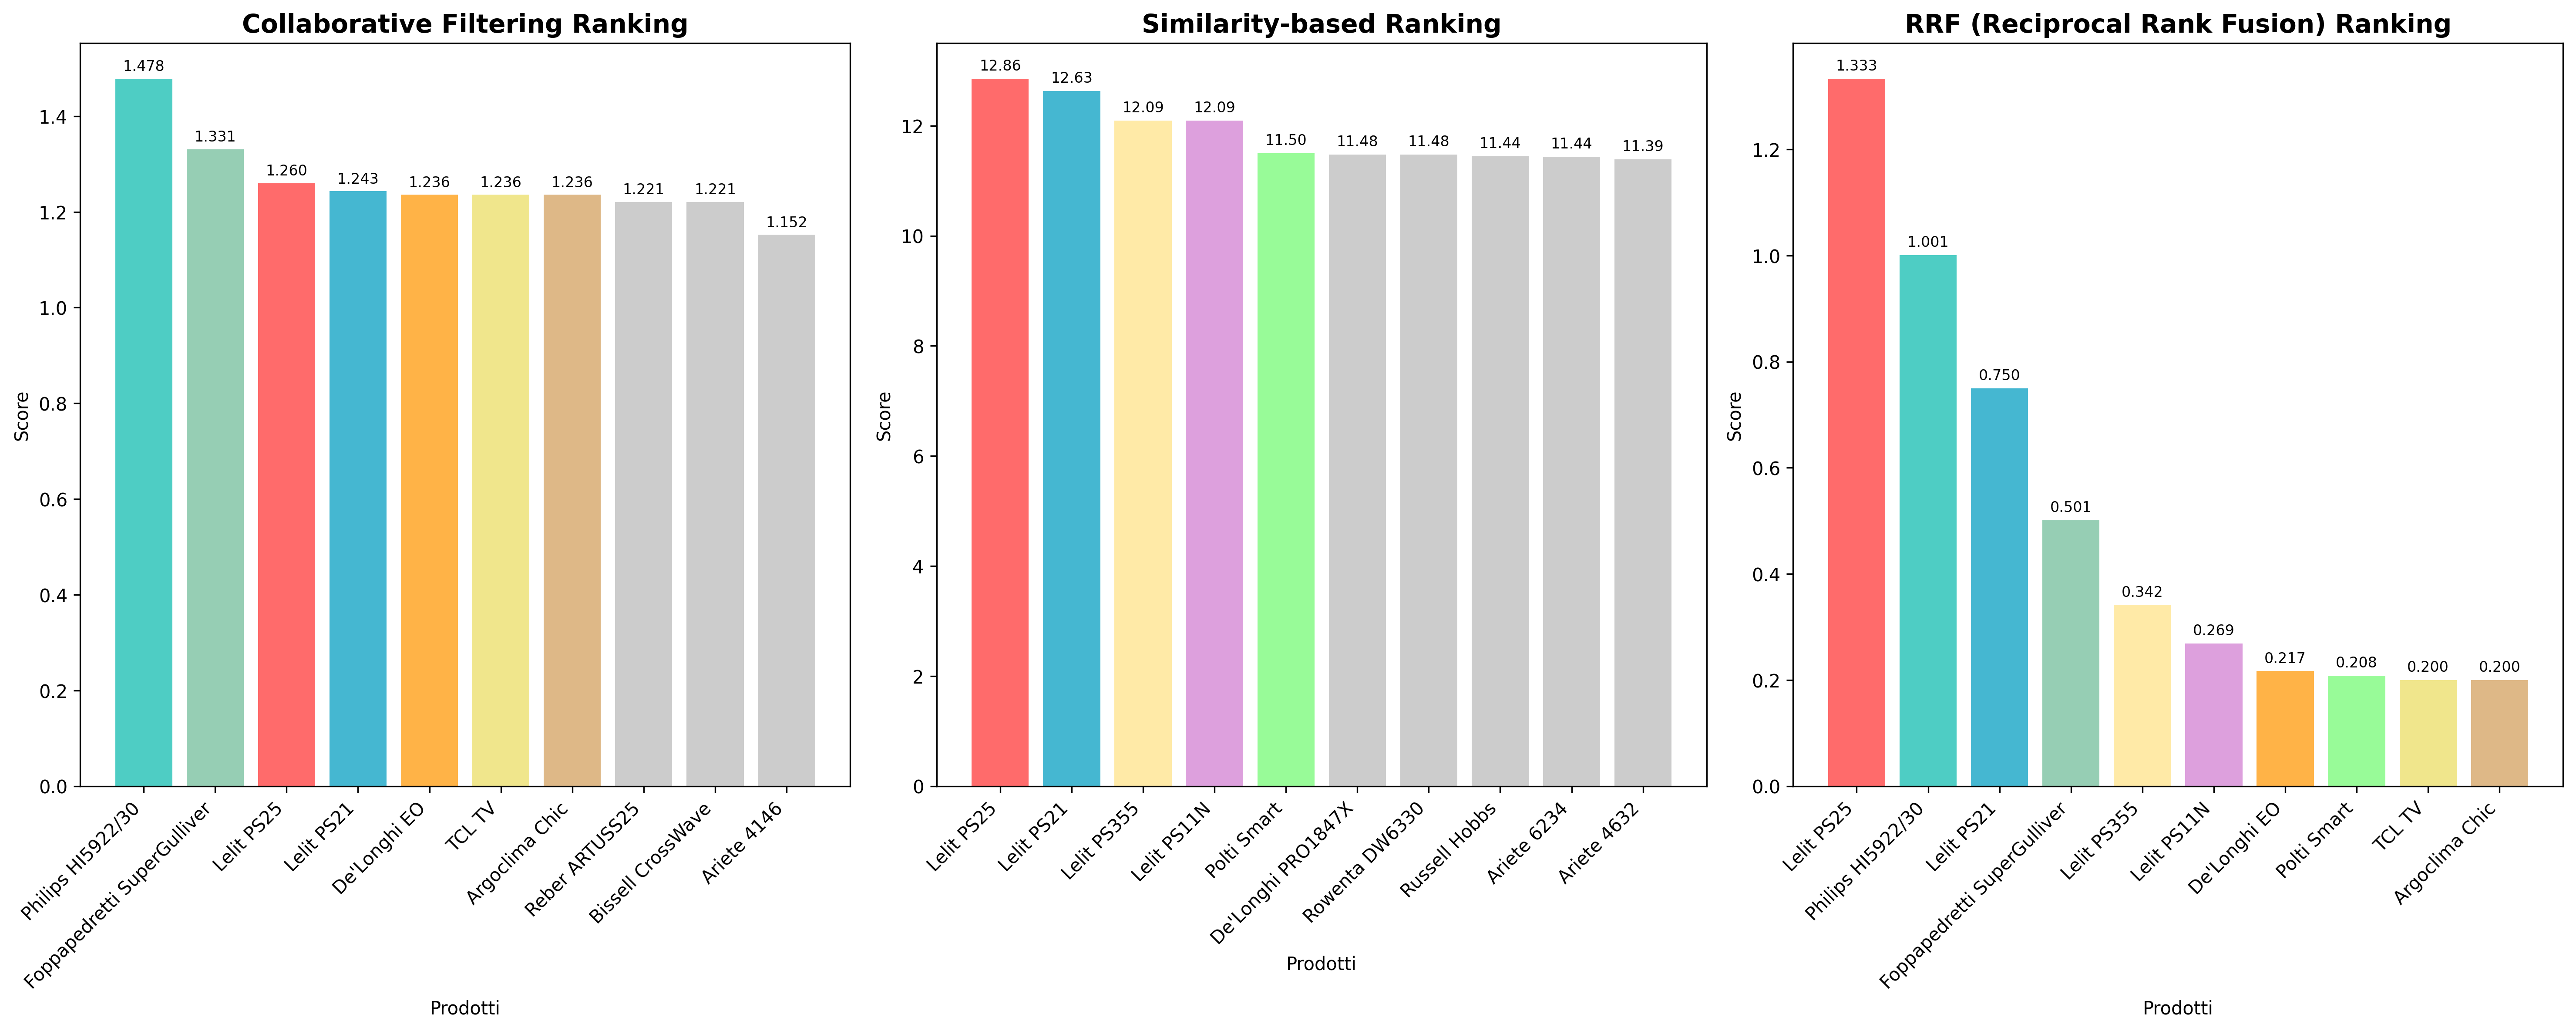
\includegraphics[width=0.8\textwidth]{rrf comparison charts/rrf_comparison_charts_real_case.png}
    \caption{Esempio di Rank Fusion con RRF su un caso reale}
    \label{fig:rank-fusion-real-case}
\end{figure}

Qui, si può notare come siano stati colorati tutti i prodotti presenti nel ranking RRF, ma, a differenza del caso giocattolo, questi prodotti non sono tutti visualizzati contemporaneamente in entrambi i due rankings di partenza, poichè il dataset contiene molto più di 10 prodotti, che è il limite di rappresentazione dei rankings in questi grafici, e quindi alcuni sono stati classificati più indietro. Inoltre, in questi due rankings originali sono visualizzati dei prodotti che non sono poi visualizzati nel ranking RRF finale, ed allora sono rimasti di colore grigio, per indicare che non sono stati raccomandati al cliente.

Il numero di raccomandazioni che il sistema restituisce viene configurato tramite apposito input dell'utente. In entrambi gli esempi mostrati, il numero di raccomandazioni è stato impostato a 10, ma questo appunto può essere modificato a piacimento.


\section{Filtro}

Una volta ottenuto il ranking finale dei prodotti, si è pensato che il sistema di raccomandazione potesse essere ulteriormente migliorato applicando un filtro sui prodotti raccomandati. È stato infatti osservato che il sistema raccomandava principalmente prodotti già acquistati dal cliente, e che questo poteva essere un problema, poichè il cliente potrebbe essere interessato a prodotti nuovi o diversi da quelli già acquistati. Per questo motivo, si è deciso di implementare un filtro che esclude i prodotti già acquistati dal cliente dalle raccomandazioni.

Questo filtro viene applicato dopo il processo di Rank Fusion, e dunque i prodotti già acquistati dal cliente vengono rimossi dal ranking finale dei prodotti raccomandati, e i prodotti raccomandati più in basso scalano di conseguenza più in alto nella classifica. In questo modo, il sistema di raccomandazione restituisce solo prodotti nuovi o diversi da quelli già acquistati, aumentando la varietà delle raccomandazioni e migliorando l'esperienza dell'utente.


\section{Confronto con RecBole e Surprise}

Una volta implementato il sistema di raccomandazione, si è pensato di confrontare le sue prestazioni con quelle di altri sistemi di raccomandazione già esistenti, ed eventualmente di prendere spunto da questi per implementare dei miglioramenti.
Per fare ciò, dopo una breve ricerca, si è deciso di utilizzare due librerie di Python per la creazione di sistemi di raccomandazione:
\begin{itemize}
    \item \textbf{\gls{recbole}}\footcite{site:recbole}: Una libreria open-source per la creazione di sistemi di raccomandazione basati su deep learning;
    \item \textbf{\gls{surprise}}\footcite{site:surprise}: Una libreria open-source per la creazione di sistemi di raccomandazione basati su metodi tradizionali come il Collaborative Filtering e la Similarità.
\end{itemize}

Per svolgere il confronto, è stato scelto un dataset, ovvero \texttt{orders\_export.csv}, e un suo cliente, ovvero \texttt{Ds-trading srl Ds-trading GmbH}, e si è proceduto a creare un sistema di raccomandazione con entrambe le librerie, utilizzando gli stessi dati di input e le stesse tecniche di raccomandazione. In particolare, per \emph{recbole} è stato utilizzato il metodo \texttt{BPR} (Bayesian Personalized Ranking), che è un algoritmo di Collaborative Filtering basato su matrice di interazioni, mentre per \emph{surprise} è stato utilizzato il metodo \texttt{KNNBasic} (K-Nearest Neighbors), che è un algoritmo di Collaborative Filtering basato su similarità tra utenti o prodotti.

Segue l'immagine \ref{fig:recbole-surprise-orders-export} degli acquisti (o interazioni) del cliente \texttt{Ds-trading srl Ds-trading GmbH}:

\newpage

\begin{figure}[h]
    \centering
    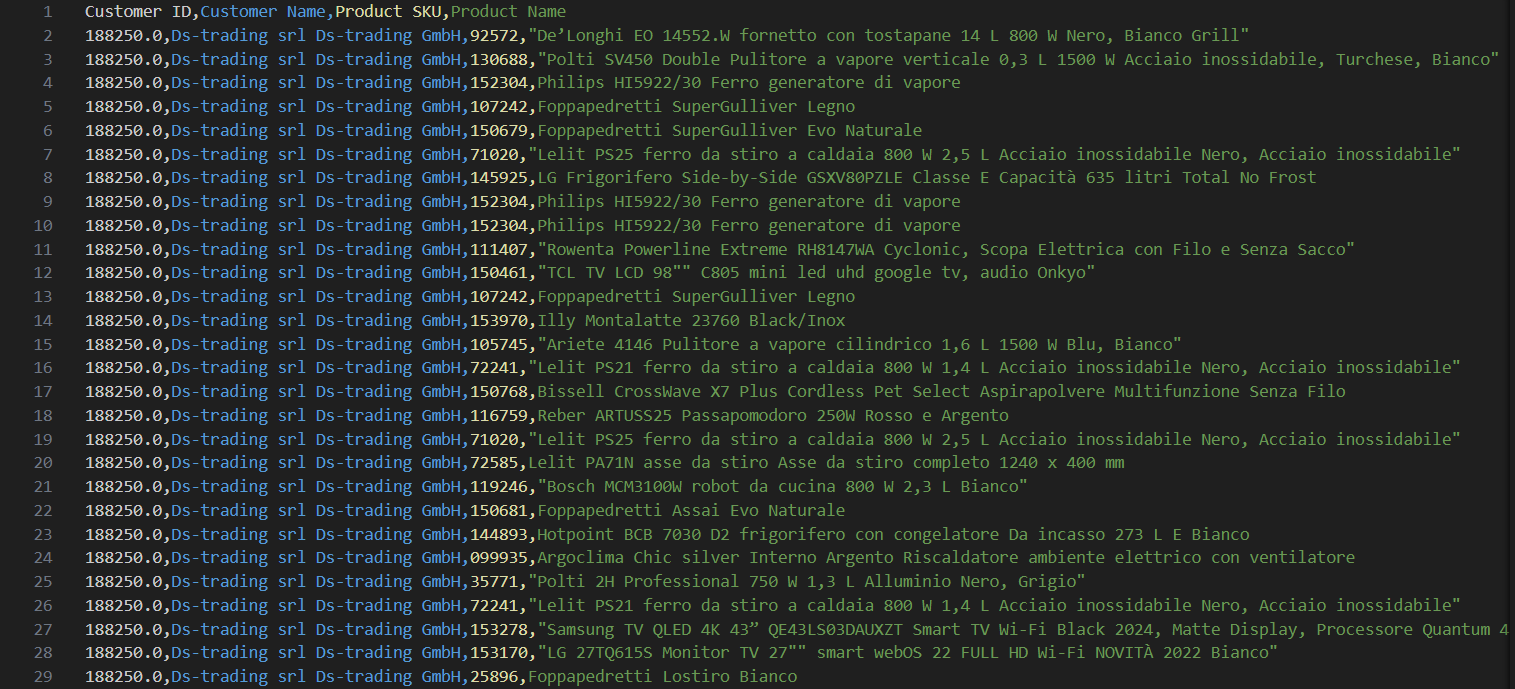
\includegraphics[width=0.8\textwidth]{recbole surprise comparison/Ds-trading purchased products.png}
    \caption{Acquisti del cliente Ds-trading srl Ds-trading GmbH}
    \label{fig:recbole-surprise-orders-export}
\end{figure}

Si può notare come il cliente abbia acquistato prettamente ferri da stiro, pulitori a vapore o riscaldatori d'ambiente, e dunque il sistema di raccomandazione dovrebbe raccomandare prodotti simili a questi, come ad esempio prodotti per la casa o elettrodomestici.

Il sistema di raccomandazione sviluppato durante lo stage raccomanda i seguenti prodotti al cliente \texttt{Ds-trading srl Ds-trading GmbH}, mostrati in figura \ref{fig:our-system-recommendations}:

\begin{figure}[h]
    \centering
    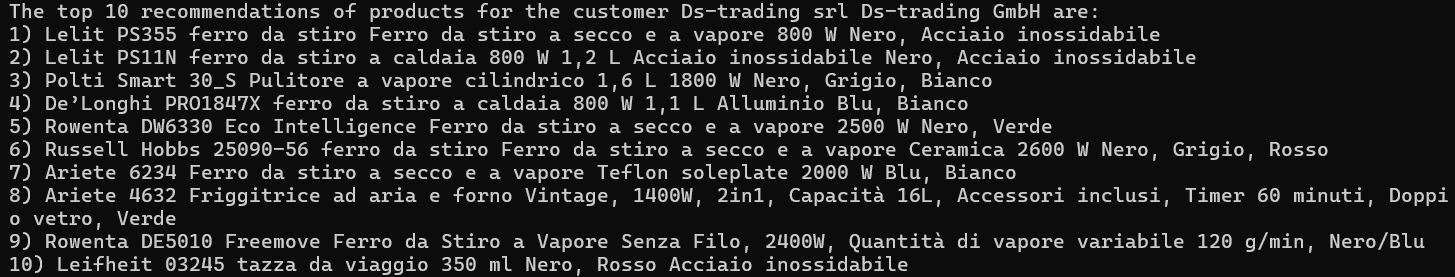
\includegraphics[width=0.8\textwidth]{recbole surprise comparison/Our system prediction.png}
    \caption{Raccomandazioni del sistema di raccomandazione sviluppato durante lo stage}
    \label{fig:our-system-recommendations}
\end{figure}

Si può notare come il sistema abbia consigliato prodotti simili a quelli già acquistati dal cliente, prettamente ferri da stiro e pulitori a vapore, che dimostrano che la similarità tra i nomi dei prodotti ha avuto un forte impatto nelle raccomandazioni. Come previsto, questo sistema lascia poco spazio alla serendipità, siccome solamente due prodotti in fondo al ranking, la friggitrice e la tazza, non sono direttamente collegati al cliente. Quest'ultima è stata una scelta implementativa chiara, poichè si è voluto creare un sistema di raccomandazione che fosse il più possibile pertinente per il cliente, e dunque che raccomandasse prodotti simili a quelli già acquistati.

Per quanto riguarda \emph{RecBole}, il sistema, prima di poter svolgere le predizioni, ha dovuto essere addestrato sui dati del cliente tramite l'algoritmo \emph{BPR}. L'immagine \ref{fig:recbole-training-outcome} rappresenta la parte finale dell'esito del training.

\newpage

\begin{figure}[h]
    \centering
    \includegraphics[width=0.8\textwidth]{recbole surprise comparison/RecBole Training.png}
    \caption{Esito di training del sistema RecBole}
    \label{fig:recbole-training-outcome}
\end{figure}

Si può notare come il training, pur avendo avuto successo, abbia mantenuto al suo termine un punteggio di loss molto alto (non è mai sceso sotto il 5), che indica che il sistema non è riuscito a generalizzare bene sui dati. Inoltre, il validation score non è mai riuscito a superare l'11\%, che è un punteggio assai basso, sia per quanto riguarda la metrica \gls{recallatk}, sia per quanto riguarda \gls{ndcgatk}. Questo è stato attribuito al fatto che nei dataset disponibili sono presenti molti clienti occasionali che non hanno interagito con un numero sufficiente di prodotti per poter fare raccomandazioni significative, e questo ha messo in crisi il sistema di raccomandazione di \emph{RecBole} basato prettamente su Collaborative Filtering.

Una volta addestrato, il sistema ha restituito le seguenti raccomandazioni per il cliente \texttt{Ds-trading srl Ds-trading GmbH}, mostrate in figura \ref{fig:recbole-recommendations}:

\begin{figure}[h]
    \centering
    \includegraphics[width=0.8\textwidth]{recbole surprise comparison/RecBole prediction.png}
    \caption{Raccomandazioni del sistema RecBole}
    \label{fig:recbole-recommendations}
\end{figure}

I risultati ottenuti da \emph{RecBole} sono stati deludenti, poichè il sistema ha raccomandato prodotti che non sono affatto simili a quelli già acquistati dal cliente, come ad esempio macchine per caffè, robot aspirapolvere o fornelli. Questi prodotti non sono pertinenti per il cliente, che ha acquistato principalmente ferri da stiro, pulitori a vapore e riscaldatori d'ambiente. Si ricorda, inoltre, che il sistema di raccomandazione sviluppato durante lo stage ha dimostrato che sono disponibili molti ferri di stiro e pulitori a vapore in vendita ma non ancora acquistati dal cliente, quindi \emph{RecBole} avrebbe dovuto consigliarne almeno uno, ma non lo ha fatto. Si è reputato dunque che il sistema di \emph{RecBole} non abbia colto correttamente le preferenze del cliente.

Per quanto riguarda \emph{Surprise}, il sistema, una volta addestrato l'algoritmo \emph{KNNBasic}, ha restituito le seguenti raccomandazioni per il cliente \texttt{Ds-trading srl Ds-trading GmbH}, mostrate in figura \ref{fig:surprise-recommendations}:

\begin{figure}[h]
    \centering
    \includegraphics[width=0.8\textwidth]{recbole surprise comparison/Surprise prediction.png}
    \caption{Raccomandazioni del sistema Surprise}
    \label{fig:surprise-recommendations}
\end{figure}

I risultati ottenuti da \emph{Surprise} sono stati ancora più deludenti, poichè il sistema ha raccomandato prodotti che non sono affatto simili a quelli già acquistati dal cliente, come ad esempio degli anni di garanzia, una fotocamera, e dei set di pentole. Ciò è stato attribuito al fatto che \emph{Surprise} richiede una colonna di rating per poter funzionare, e questa colonna non è presente nei dataset disponibili. Per fare il confronto, era stata creata una colonna di rating fittizia, che assegnava un rating fisso di 1 a ciascun acquisto, ma questo ha portato a risultati inutilizzabili, poichè ogni raccomandazione viene considerata perfetta, e dunque il sistema non riesce a distinguere tra prodotti buoni e cattivi. Infatti, come si vede in figura \ref{fig:surprise-recommendations}, a seguire la scritta \texttt{Stima: } è sempre presente il valore \texttt{1.00}, che indica che il sistema ha assegnato un punteggio di 1 a tutti i prodotti del dataset, e quindi non è più in grado di fare distinzioni tra di essi. Si è reputato dunque che il sistema di \emph{Surprise} non fosse adatto al caso in esame, che non prevede l'esistenza di rating.

Al termine del confronto, si è dunque deciso di non considerare alcun contributo dalle librerie \emph{RecBole} e \emph{Surprise} per il sistema di raccomandazione, poichè i risultati da esse ottenuti non erano soddisfacenti ed erano assai peggiori rispetto ai risultati ottenuti dal sistema implementato. Tuttavia, queste librerie possono essere utili per ulteriori sperimentazioni e per la creazione di sistemi di raccomandazione più avanzati in futuro.


\section{Serendipità}

Un tema di ricerca interessante nel campo dei sistemi di raccomandazione è la \textbf{Serendipità}. Questo concetto si riferisce alla capacità del sistema di raccomandare prodotti inaspettati ma potenzialmente interessanti per l'utente, che potrebbero non essere stati considerati in precedenza. La Serendipità è un aspetto importante dei sistemi di raccomandazione, poiché può migliorare l'esperienza dell'utente e aumentare la soddisfazione del cliente.

A riguardo, è stato letto l'articolo \emph{Serendipity in Recommender Systems: A Systematic Literature Review}\footcite{article:serendipity-recommender-systems}, pubblicato dall'Università di Teheran, che fornisce una panoramica completa della Serendipità nei sistemi di raccomandazione. L'articolo analizza le definizioni, le metriche e le tecniche utilizzate per misurarla e implementarla. Viene evidenziato come la Serendipità possa essere vista sia come un obiettivo di ricerca, sia come un aspetto pratico da considerare nella progettazione dei sistemi di raccomandazione.

Nel contesto del progetto, la Serendipità è stata considerata come un obiettivo di ricerca, ma non è stata implementata nello stato dell'arte del sistema di raccomandazione, per mancanza di tempo e di dataset adatti a testarla. Tuttavia, si è pensato che la Serendipità potesse essere un aspetto interessante da esplorare in futuro, e che potesse essere implementata come un ulteriore filtro sui prodotti raccomandati, per escludere quelli già noti o attesi dall'utente e favorire quelli inaspettati.


\section{Metriche}
\label{sec:metrics}

Il sistema di raccomandazione implementato è stato valutato utilizzando diverse metriche\footcite{site:metrics-recommender-systems}, che sono state scelte in base agli obiettivi del progetto e alle caratteristiche del dataset.

Molte metriche utilizzano la rilevanza come criterio di valutazione, e dunque è necessario definire cosa si intende per "item rilevante". Nel contesto del progetto, un "item rilevante" è un prodotto che è stato acquistato dal cliente. Tuttavia, il sistema di raccomandazione non raccomanda nessun item che è stato acquistato dal cliente, poiché questi vengono filtrati. Dunque, le metriche sono state classificate in due categorie:
\begin{itemize}
    \item \textbf{Metriche pre-filtro}: metriche che valutano le raccomandazioni prima dell'applicazione del filtro sui prodotti già acquistati dal cliente; appartengono a questa categoria le metriche che considerano gli "item rilevanti" come mezzo di valutazione del ranking;
    \item \textbf{Metriche post-filtro}: metriche che valutano le raccomandazioni dopo l'applicazione del filtro sui prodotti già acquistati dal cliente; appartengono a questa categoria le metriche che non utilizzano gli "item rilevanti" come mezzo di valutazione del ranking.
\end{itemize}

Le metriche pre-filtro utilizzate sono:
\begin{itemize}
    \item \textbf{\gls{recallatk}}\footcite{site:recall}: misura la frazione di elementi rilevanti recuperati tra i primi $k$ risultati restituiti dal sistema di raccomandazione, rispetto al totale degli elementi rilevanti disponibili per l'utente;
    \item \textbf{\gls{precisionatk}}\footcite{site:precision_at_k}: misura la frazione di elementi rilevanti tra i primi $k$ risultati restituiti dal sistema di raccomandazione;
    \item \textbf{\gls{mapatk}}\footcite{site:mean_average_precision}: calcola la media delle precisioni valutate a ogni posizione in cui un elemento rilevante appare tra i primi $k$ risultati, fornendo una misura globale della qualità del ranking;
    \item \textbf{\gls{mrratk}}\footcite{site:mean_reciprocal_rank}: calcola la media dei reciproci della posizione degli elementi rilevanti tra i primi $k$ risultati, privilegiando i risultati rilevanti in posizioni più alte;
    \item \textbf{\gls{unserendipityatk}}\footcite{article:serendipity-recommender-systems}: misura la mancanza di serendipità tra i primi $k$ risultati, ovvero la tendenza del sistema a raccomandare elementi già noti o attesi dall'utente piuttosto che scoperte inaspettate.
\end{itemize}

Mentre, le metriche post-filtro utilizzate sono:
\begin{itemize}
    \item \textbf{\gls{averageitemsimilarity}}\footcite{site:average_item_similarity}: calcola la media delle similarità tra gli elementi raccomandati e gli elementi con cui l'utente ha già interagito, fornendo una misura della diversità delle raccomandazioni;
    \item \textbf{\gls{meanpopularityatk}}\footcite{article:mean_popularity}: misura la media della popolarità degli elementi raccomandati tra i primi $k$ risultati, dove la popolarità è determinata dal numero totale di interazioni ricevute da ciascun elemento nel dataset.
\end{itemize}

Le metriche sono state scelte in base agli obiettivi del progetto e alle caratteristiche del dataset. In particolare, le metriche pre-filtro sono state scelte per valutare la qualità delle raccomandazioni in base a quanti item rilevanti sono stati recuperati tra i primi $k$ risultati, mentre le metriche post-filtro sono state scelte per valutare la qualità delle raccomandazioni in base alla similarità e alla popolarità degli item raccomandati.

Le metriche che erano state inizialmente valutate, ma che poi sono state scartate, sono:
\begin{itemize}
    \item \textbf{\gls{ndcgatk}}\footcite{site:ndcg}: calcola il guadagno cumulativo scontato normalizzato, che tiene conto sia della rilevanza degli elementi sia della loro posizione nel ranking tra i primi $k$ risultati;
    \item \textbf{\gls{hitrateatk}}\footcite{site:hit_rate}: metrica binaria che vale 1 se almeno un elemento rilevante è presente tra i primi $k$ risultati raccomandati, 0 altrimenti;
    \item \textbf{\gls{coverageatk}}\footcite{site:coverage_metric}: misura la varietà del sistema calcolando quanti elementi diversi vengono raccomandati complessivamente agli utenti tra i primi $k$ risultati;
    \item \textbf{\gls{intralistdiversity}}\footcite{article:diversity_metric}: misura quanto sono diversi tra loro gli elementi raccomandati all'interno della stessa lista di raccomandazioni;
    \item \textbf{\gls{novelty}}\footcite{site:novelty_metric}: quantifica la novità delle raccomandazioni favorendo elementi poco popolari, che sono potenzialmente più "nuovi" per l'utente.
\end{itemize}

Queste metriche sono state scartate per diverse ragioni metodologiche e concettuali. La metrica \emph{nDCG@k} è stata considerata ridondante rispetto alla Recall@k, poiché nel contesto specifico del progetto la posizione esatta degli elementi rilevanti nel ranking ha un'importanza limitata. La \emph{Hit Rate@k} è stata giudicata troppo semplicistica, fornendo solo un'informazione binaria sulla presenza di almeno un elemento rilevante senza considerare la qualità complessiva delle raccomandazioni.

Per quanto riguarda le metriche \emph{Coverage@k}, \emph{Intra-list Diversity} e \emph{Novelty}, queste sono state escluse poiché il sistema di raccomandazione implementato non è stato progettato per massimizzare la diversità o la novità delle raccomandazioni. Al contrario, il sistema si basa su tecniche di Collaborative Filtering e Similarità che tendono naturalmente a raccomandare elementi simili a quelli già acquistati dall'utente. L'applicazione di queste metriche avrebbe inevitabilmente prodotto punteggi molto bassi, non fornendo informazioni utili sulla qualità del sistema. Per questo motivo, si è preferito utilizzare la sovraccitata metrica \emph{Unserendipity@k}, che misura l'opposto della serendipità\footcite{site:serendipity} e risulta dunque più appropriata per valutare un sistema orientato alla similarità e alla coerenza delle raccomandazioni.

La metrica \emph{Unserendipity@k} è stata scelta tra le metriche presentate nell'articolo \emph{Serendipity in Recommender Systems: A Systematic Literature Review}\footcite{article:serendipity-recommender-systems} riguardanti la Serendipità, poiché si è ritenuto che fosse la più adatta tra le metriche di Serendipità per valutare un sistema di raccomandazione basato sulla Similarità.
Le altre metriche considerate nell'articolo erano le seguenti:
\begin{itemize}
    \item \textbf{\gls{serendipity}}\footcite{site:serendipity_metric}: misura la capacità del sistema di raccomandare elementi inaspettati ma potenzialmente interessanti per l'utente;
    \item \textbf{\gls{surprise_metric}}\footcite{article:surprise_metric}: quantifica il grado di sorpresa nelle raccomandazioni calcolando la distanza tra le aspettative dell'utente e i risultati effettivi;
    \item \textbf{\gls{confidence}}\footcite{article:confidence_metric}: valuta il livello di fiducia del sistema nelle proprie raccomandazioni, spesso correlato alla popolarità degli elementi;
    \item \textbf{\gls{distance}}\footcite{site:distance_measures}: misura la distanza semantica o comportamentale tra gli elementi raccomandati e quelli già noti all'utente;
    \item \textbf{\gls{expectedness}}\footcite{article:expectedness}: quantifica quanto le raccomandazioni siano prevedibili o attese dall'utente;
    \item \textbf{\gls{rmse}}: calcola l'errore quadratico medio per valutare l'accuratezza delle predizioni di rating.
\end{itemize}

Tuttavia, queste metriche non sono state considerate appropriate per il contesto specifico del sistema implementato. Le metriche \emph{Serendipity}, \emph{Surprise} e \emph{Confidence} si basano principalmente su concetti di rilevanza e popolarità che non si allineano con gli obiettivi del sistema. La rilevanza, infatti, perde significato nel momento in cui viene applicato il filtro che esclude i prodotti già acquistati, rendendo questa dimensione di valutazione non pertinente per il ranking finale presentato all'utente. Allo stesso modo, la popolarità non rappresenta un criterio di interesse per il sistema implementato, poiché l'obiettivo non è raccomandare prodotti universalmente apprezzati, bensì prodotti specificamente adatti alle preferenze e al profilo del singolo cliente.

Le metriche \emph{Distance} ed \emph{Expectedness}, pur essendo concettualmente interessanti, non forniscono un'adeguata rappresentazione della qualità delle raccomandazioni in un contesto dove l'obiettivo è identificare prodotti semanticamente coerenti con le preferenze dell'utente. Infine, la metrica \emph{RMSE} non è applicabile al sistema implementato poiché questo non predice rating numerici espliciti.

Al contrario, la metrica \emph{Unserendipity@k} è stata selezionata proprio perché si basa sulla similarità semantica tra i prodotti, allineandosi perfettamente con la filosofia del sistema implementato. Questa metrica valuta la coerenza delle raccomandazioni rispetto ai pattern di acquisto dell'utente, misurando quanto il sistema sia efficace nel mantenere una linea di coerenza tematica nelle sue proposte. Tale approccio risulta particolarmente appropriato per un sistema di e-commerce dove l'obiettivo primario è suggerire prodotti che si integrino naturalmente con le preferenze già manifestate dal cliente, piuttosto che sorprenderlo con scelte completamente inaspettate.


\section{Explainability}

Un requisito opzionale del sistema di raccomandazione implementato era la \textbf{\gls{explainability}}\footcite{site:explainable-ai} delle raccomandazioni. Questo aspetto è stato considerato importante poiché consente agli sviluppatori e manutentori del sistema di comprendere le ragioni dietro le raccomandazioni fornite dal sistema, consentendo di identificare eventuali problemi o miglioramenti da apportare al sistema stesso.

La explainability prevede di esplicare i procedimenti e le logiche che portano il sistema a raccomandare determinati prodotti, rendendo trasparente il processo decisionale del sistema. Nel contesto del sistema di raccomandazione implementato, l'ultimo livello raggiunto prima di raccomandare i prodotti è il \emph{rank fusion}, che combina i risultati dei due sistemi di raccomandazione (Collaborative Filtering e Similarità) in un unico ranking finale. Per rendere il sistema spiegabile, si è dunque scelto di fornire le informazioni sui ranking dei due sistemi di raccomandazione che hanno contribuito alla generazione del ranking finale.

In particolare, per ogni prodotto raccomandato, il sistema stampa su console, tramite la libreria \gls{logging}, le seguenti informazioni:
\begin{itemize}
    \item Il ranking ed il punteggio RRF del prodotto;
    \item Il ranking ed il punteggio del prodotto nel sistema di Collaborative Filtering;
    \item Il ranking del prodotto nel sistema di Similarità.
\end{itemize}

Queste informazioni consentono di comprendere come il prodotto è stato classificato nei due sistemi di raccomandazione e come questi ranking sono stati combinati per generare il ranking finale. In questo modo, gli sviluppatori e manutentori del sistema possono avere una visione chiara delle logiche che portano il sistema a raccomandare determinati prodotti, e possono identificare eventuali problemi o miglioramenti da apportare al sistema stesso.

Erano stati pensati anche altri metodi per rendere il sistema spiegabile, cioè i seguenti:
\begin{itemize}
    \item \textbf{Visualizzazione dei ranking}: Creare una visualizzazione grafica dei ranking dei due sistemi di raccomandazione, in modo da mostrare come i prodotti sono stati classificati nei due sistemi e come questi ranking sono stati combinati per generare il ranking finale;
    \item \textbf{Analisi delle interazioni}: Fornire informazioni sulle interazioni degli utenti con i prodotti, in modo da spiegare perché la matrice di collaborative filtering ha raccomandato determinati prodotti;
    \item \textbf{Analisi delle similarità}: Fornire informazioni sulle similarità tra i prodotti raccomandati e i prodotti già acquistati dal cliente, in modo da spiegare perché la matrice di similarità ha raccomandato determinati prodotti.
\end{itemize}

La visualizzazione dei ranking è stata scartata poichè la piattaforma \gls{googlecloudfunctions} non supporta la visualizzazione grafica dei dati, e dunque non sarebbe stato possibile implementarla. Si è dunque deciso di mantenere solo la stampa su console dei ranking e dei punteggi, appunto l'unica possibile sulla piattaforma, che è comunque un metodo di visualizzazione efficace per rendere il sistema spiegabile.

Per quanto riguarda l'analisi delle interazioni e delle similarità, queste sono state considerate troppo complesse da implementare e avrebbero richiesto un ulteriore livello di complessità e di elaborazione dei dati, che non era previsto nel progetto.
Si è dunque deciso di mantenere la spiegabilità solamente del sistema di \emph{rank fusion}, delegando agli sviluppatori e manutentori del sistema la responsabilità di comprendere le logiche dei due sistemi di raccomandazione sottostanti.
